\documentclass[a4paper, 12pt]{article} % тип документа

%%%Библиотеки
	%\usepackage[warn]{mathtext}	
	\usepackage[T2A]{fontenc}   %Кодировка
	\usepackage[utf8]{inputenc} %Кодировка исходного текста
	\usepackage[english, russian]{babel} %Локализация и переносы
	\usepackage{caption}
	\usepackage{listings}
	\usepackage{amsmath, amsfonts, amssymb, amsthm, mathtools}
	\usepackage[warn]{mathtext}
	\usepackage[mathscr]{eucal}
	\usepackage{wasysym}
	\usepackage{graphicx} %Вставка картинок правильная
	\DeclareGraphicsExtensions{.pdf,.png,.jpg}
	\graphicspath{ {images/} }
	
	\setlength{\parskip}{0.5cm}
	
	\usepackage{pgfplots}
	\usepackage{indentfirst}
	\usepackage{float}    %Плавающие картинки
	\usepackage{wrapfig}  %Обтекание фигур (таблиц, картинок и прочего)
	\usepackage{fancyhdr} %Загрузим пакет
	\usepackage{lscape}
	\usepackage{xcolor}
	\usepackage[normalem]{ulem}
	\usepackage{wasysym}
	\usepackage{subfig}
	\usepackage{graphicx}
	
	\usepackage{titlesec}
	\titlelabel{\thetitle.\quad}

	\usepackage{hyperref}
	\newenvironment{comment}{}{}

%%%Конец библиотек

%%%Настройка ссылок
%%%	\hypersetup
%%%	{
%%%		colorlinks = true,
%%%		linkcolor  = blue,
%%%		filecolor  = magenta,
%%%		urlcolor   = blue
%%%	}
%%%Конец настройки ссылок


%%%Настройка колонтитулы
    \pagestyle{fancy}
    \fancyhead{}
    \fancyhead[L]{1.1.1}
    \fancyhead[R]{Засимов Георгий, группа Б01-109}
    \fancyfoot[C]{\thepage}
%%%конец настройки колонтитулы




%Заговолок

\begin{document}

\begin{titlepage}

    \newpage
    \begin{center}
        \normalsize Московский физико-технический институт \\(национальный исследовательский университет)
    \end{center}

    \vspace{6em}

    \begin{center}
        \Large Лабораторная работа по общему курсу физики\\
    \end{center}

    \vspace{1em}

    \begin{center}
        \Large \textbf{Отчёт о выполнении лабораторной работы 1.3.2\\ {Определение модуля сдвига при помощи крутильных колебаний.}}
    \end{center}

    \vspace{2em}

    \begin{center}
        \large Засимов Георгий Алексеевич \\
        Группа Б01-109
    \end{center}

    \vspace{\fill}

    \begin{center}
    Долгопрудный \\2021
    \end{center}
    
\end{titlepage}

\newpage

%\\\\\\\\\\\\\\\\\\\\\\\\\\\\\\\\\\\\\\\\\\\\\\\\\\\\\\\\\\\\\\\\\\\\\\\\\\\\
\section{Аннотация}

    В данной работе находим модули кручения и сдвига по крутильным колебаниям проволоки с грузами. Исследуем зависимость расстояния от оси вращения до грузов от периода колебаний. Сравниваем полученное значение с табличным и определяем материал проволоки.



%----------------------------------------------------
\section{Теоретические сведения и методика измерений}

    При закручивании цилиндрических стержней круглого сечения распределение деформаций и напряжений одинаково по длине стержня только вдали от мест где прикладываются закручивающие моменты. Для этих областей можно считать, что каждое поперечное сечение поворачивается как жесткое. Возникающее при этом напряженное состояние - чистое кручение. Рассматриваем тонкие кольца части цилиндра бесконечно малой длины $dl$, образующая которого наклоняется на малый угол $\alpha$, а верхнее сечение смещается на $d\phi$ относительно нижнего. Касательное напряжение $\tau = G\alpha$ зависит от модуля сдвига $G$.
    
    Связь приложенного момента сил $M$ и угла поворота поперечных сечений цилиндра $\phi$, находящихся на расстоянии $l$ имеет вид:
    
\begin{equation} \label{момент сил}
    M = \frac{\pi R^4 G}{2l}\phi = f\phi
\end{equation}

    где $f$ - модуль кручения:
    
\begin{equation} \label{модуль кручения ф}
    f = \frac{\pi R^4 G}{2l}
\end{equation}



%-----------------------------------------------------
\section{Оборудование и экспериментальные погрешности}


%---------------------------------------
\subsection{Экспериментальная установка и методика измерений}

    Схема экспериментальной установки представлена на рис. 1. (П - проволока, С - стержень, Г - груз).
    
\begin{center}
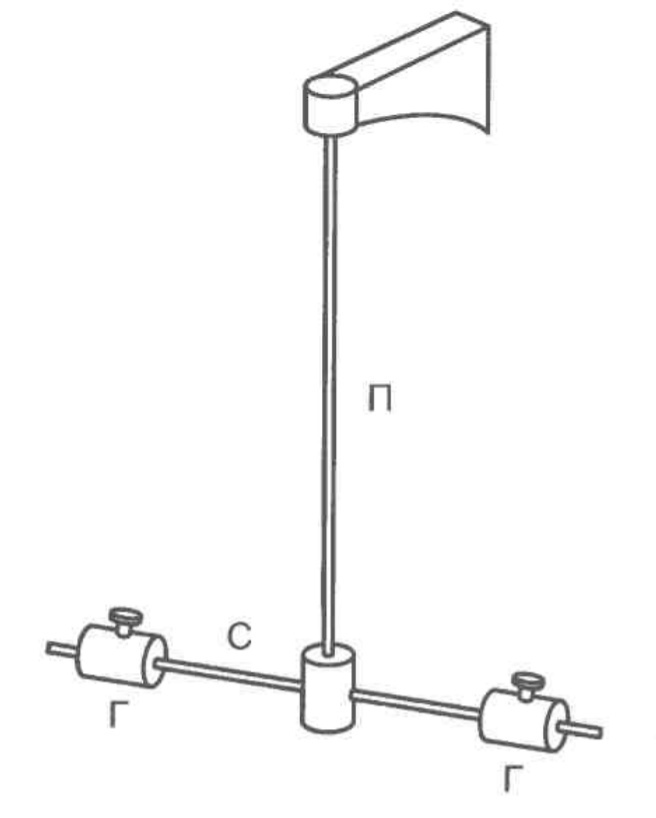
\includegraphics[width=6cm, height=9cm]{coleb.jpeg}
\end{center}
\begin{flushright}
{\scriptsize \textbf{Рис. 1.} \textbf {Экспериментальная установка.}}
\end{flushright}

   Вращение стержня с грузами описывается уравнением ($I$ - момент инерции стержня с грузами, $\phi$ - угол поворота стержня от положения равновесия, М - момент сил):
   
\begin{equation} \label{ур вращ стер}
    I\frac{d^2\phi}{dt^2} = -M
\end{equation}

    Получим уравнение гармонических колебаний из \eqref{момент сил} \eqref{ур вращ стер} (обозначим $\omega^2 = \frac{f}{I}$):
    
\begin{equation}
    \frac{d^2\phi}{dt^2} + \omega^2\phi = 0
\end{equation}

    Его решение имеет вид:
    
\begin{equation}
    \phi = \phi_0 Sin(\omegat + \theta)
\end{equation}


    где амплитуда $\phi$ и фаза $\theta$ определяются начальными условиями.
    
    Период колебаний равен:
    
\begin{equation} \label{период Т}
    T = \frac{2\pi}{\omega} = 2\pi \sqrt{\frac{I}{f}}
\end{equation}

    Данные формулы верны для незатухающих колебаний.
    


%---------------------------------
\subsection{Погрешности измерений}

    В данной работе используем линейку для нахождения длины проволоки ($\sigma_L$ = 10 mm)и расстояния от стержня до грузов ($\sigma_l$ = 0,5 mm), штангенциркулем для длин и диаметров цилиндров ($\sigma_{sh}$ = 0,1 mm), микрометром для диаметра проволоки ($\sigma_{mk}$ = 0,01 mm), весами для определения масс грузов ($\sigma_m$ = 0,1 g) и секундомером для определения времени колебаний ($\sigma_t$ = 0,1 c).
    
    Полученные значения с соответствующими погрешностями:
    
\[m_1 = 377,6 \pm 0,1 g (\varepsilon = 0,03\%)\]
\[m_2 = 373,4 \pm 0,1 g (\varepsilon = 0,03\%)\]

\[l_1 = 48 \pm 0,5 mm (\varepsilon = 1\%)\]
\[l_2 = 49 \pm 0,5 mm (\varepsilon = 1\%)\]

\[L = 173,8 \pm 1 cm (\varepsilon = 0,6 \%)\]

\[d = 2,44 \pm 0,01 mm (\varepsilon = 0,4\%)\]
=>
\[R = 1,22 \pm 0,01 mm (\varepsilon = 0,8\%)\]



%------------------------------------------------
\section{Результаты измерений и обработка данных}

    Результаты измерений времени колебаний стержня с грузами в зависимости от положения грузов относительно стержня с соответствующими значениями периода колебаний приведены в таблице 1.
    
\newpage
\begin{table}[h!]
\centering
\begin{tabular}{|l|l|l|l|}
\hline
l, см & N, шт & t, c  & T, c   \\ \hline
12,83 & 15    & 64,47 & 4,2980 \\ \hline
12,83 & 15    & 63,84 & 4,2560 \\ \hline
12,83 & 15    & 63,94 & 4,2627 \\ \hline
10,33 & 17    & 62,1  & 3,6529 \\ \hline
10,33 & 17    & 62,22 & 3,6600 \\ \hline
10,33 & 17    & 62,56 & 3,6800 \\ \hline
8,33  & 20    & 63,16 & 3,1580 \\ \hline
8,33  & 20    & 62,69 & 3,1345 \\ \hline
7,33  & 21    & 60,81 & 2,8957 \\ \hline
7,33  & 21    & 60,56 & 2,8838 \\ \hline
5,43  & 26    & 62,34 & 2,3977 \\ \hline
5,43  & 26    & 62,25 & 2,3942 \\ \hline
4,03  & 30    & 62,78 & 2,0927 \\ \hline
4,03  & 30    & 62,71 & 2,0903 \\ \hline
\end{tabular}
\end{table}
\begin{flushright}
{\scriptsize \textbf{Таблица 1.} \textbf {Результаты измерений.}}
\end{flushright}


    Построим график зависимости квадрата расстояния от стержня до центра масс грузов от квадрата периода колебаний (см Рис. 2).
    
    Момент инерции для пустого стержня:
    
\[I_0 = \frac{<T_0>^2}{4\pi^2}f\]

    для стержня с грузами (на расстоянии $r$ от стержня):
    
\[I = I_1 + I_0 = (m_1 + m_2)r^2 + I_0\]

    Период колебаний системы:
    
\[T^2 = \frac{4\pi^2I}{f} = \frac{4\pi^2}{f} (I_0 + (m_1 + m_2)L^2)\]
    
\newpage
\begin{center}
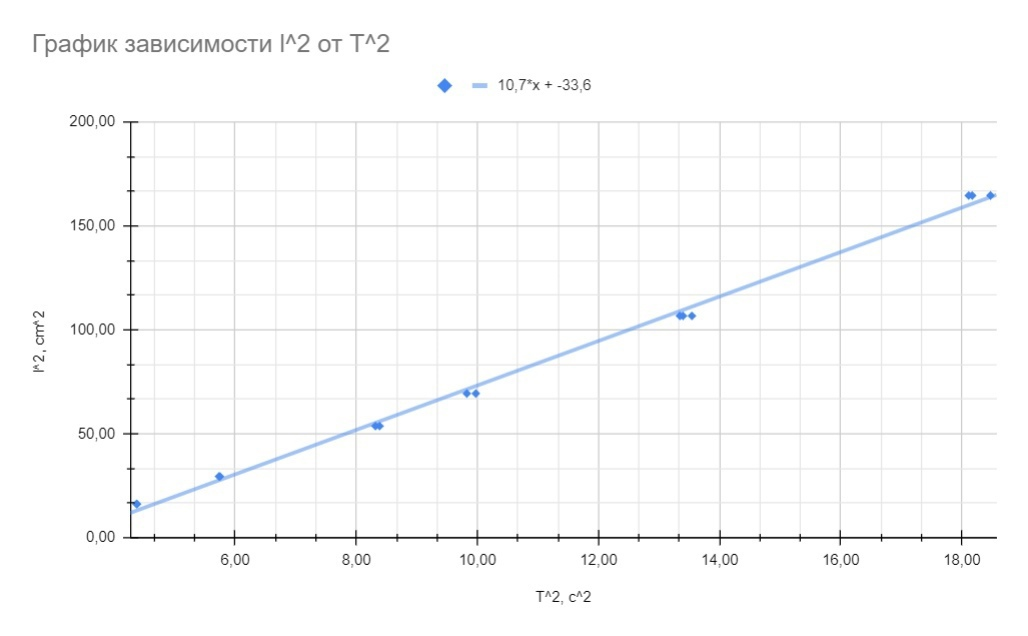
\includegraphics[width=14cm, height=9cm]{tl.jpeg}
\end{center}
\begin{flushright}
{\scriptsize \textbf{Рис. 2.} \textbf {График зависимости квадрата расстояния от стержня до грузов $l^2$ от квадрата периода колебаний $T^2$.}}
\end{flushright}
    
    Видим, что зависимость линейна, график - прямая, не проходящая через начало координат, поскольку колебания расстояния $l$ - не нулевые. По найденному по методу наименьших квадратов коэффициенту наклона прямой $k = \frac{4\pi^2 (m_1 + m_2)}{f}$ найдем модуль кручения $f$ по формуле из \eqref{период Т}:
    
\[f = \frac{4\pi^2(m_1 + m_2)}{k}\]

\[k = \frac{<xy> - <y><x>}{<x^2> - <x>^2}\]    
    
    Погрешность определения значения $k$:
    
\[\sigma_{k} = \sqrt{\frac{1}{N-1} \left(\frac{<y^2> - <y>^2}{<x^2> - <x>^2} - k^2\right)} = 14,54 c^2/m^2\]

\[k = 933 \pm 15 \frac{cm^2}{c^2}\]
\[\varepsilon_k =  1,6 \%\]

\[\varepsilon_f = \sqrt{\varepsilon_k^2 + \varepsilon_l^2 + \varepsilon_m^2} = 7,18\%\]
\[f = 0,032 \pm 0,002 \frac{m}{c^2}\]\\

    Найдем модуль сдвига $G$  из формулы \eqref{модуль кручения ф}:
    
\[G = \frac{2L f}{\pi R^4}\]

\[\varepsilon_G = \sqrt{\varepsilon_f^2 + \varepsilon_L^2 + 16\varepsilon_R^2} = 7,9\%\]

\[G = 36 \pm  3 GPa\]
    
    

%----------------
\section{Выводы}

    В данной работе мы нашли модуль сдвига исследуемого материала проволоки: $G = 36 \pm 3 $ ГПа. Основной вклад в погрешность определения модуля сдвига вносит погрешность измерения времени, расстояний от грузов до оси и нахождения радиуса проволоки. Ближе всего по табличным значениям исследуемый материал к меди (35 - 49 ГПа). Можно предположить, что проволока изготовлена из сплава меди.\\
    
    
    
\end{document}
